
\begin{frame}
\begin{block}{Vraag}
Hebben we ook 100\% effici�ntie als we een oneindig vlak zouden betegelen met cirkels?
\end{block}
%\begin{figure}[h]
 % \centering
 % \subfloat[]{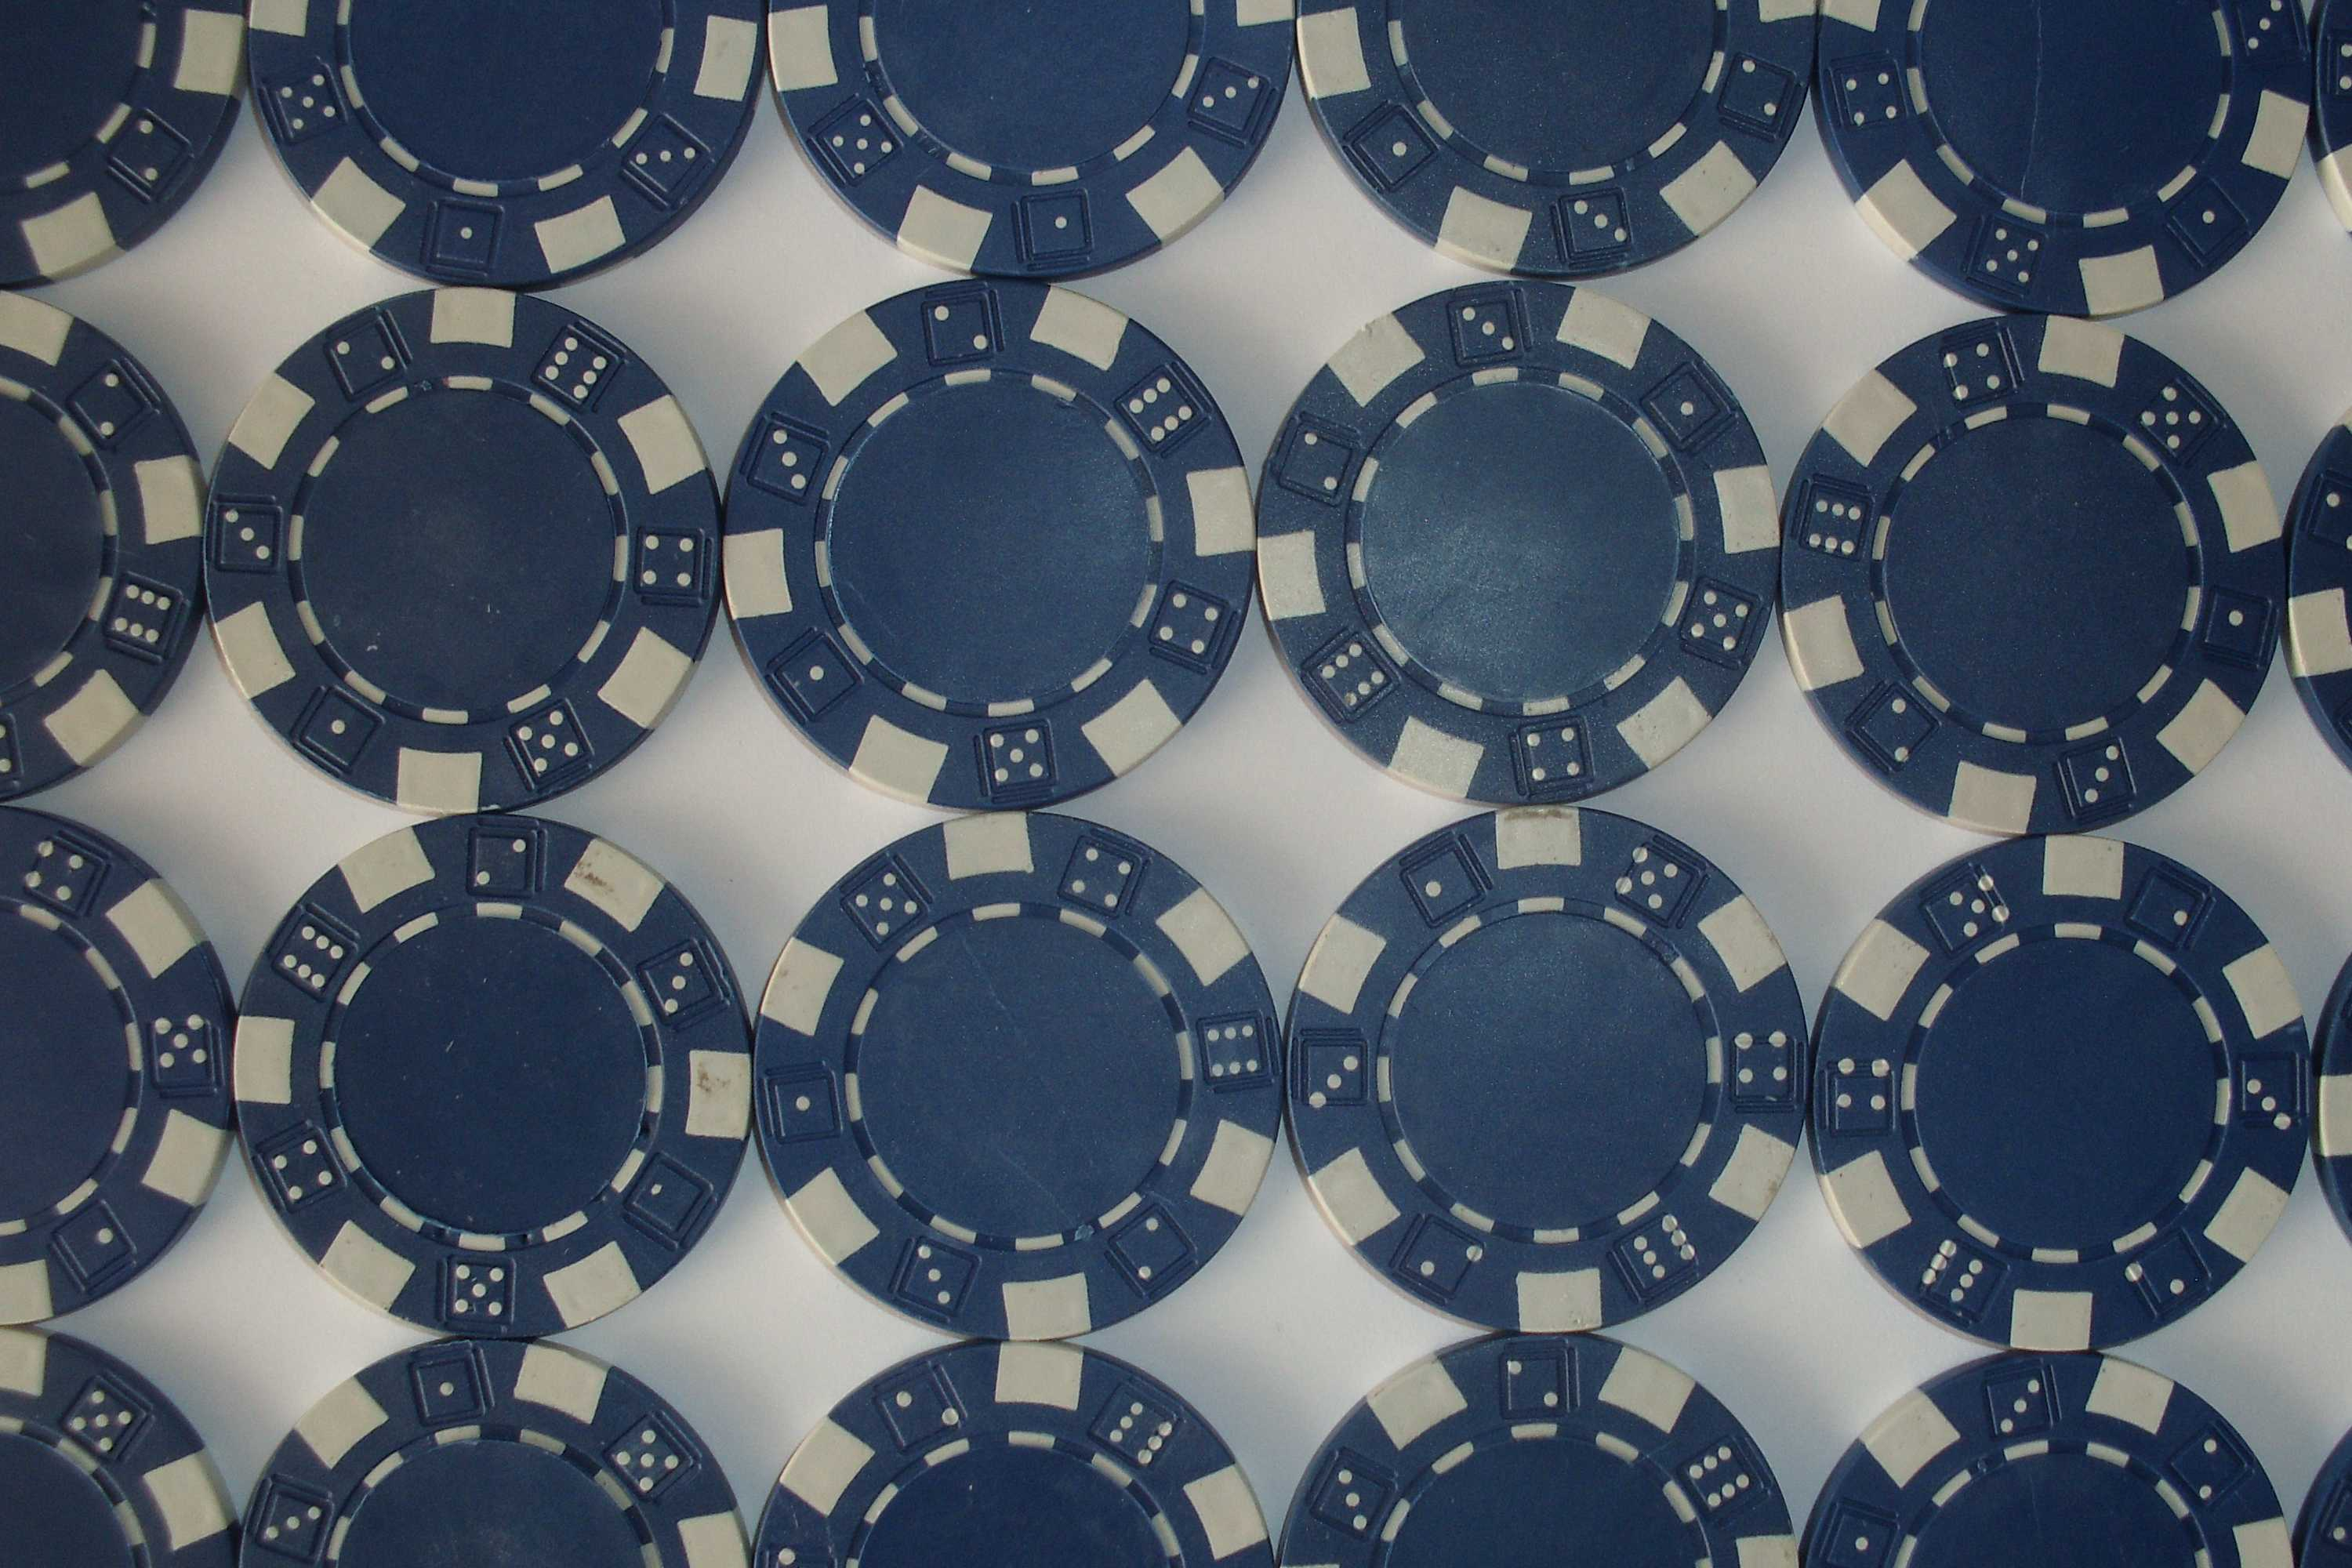
\includegraphics[height= 4cm]{jetons_sqr}\label{js}}\qquad
 % \subfloat[]{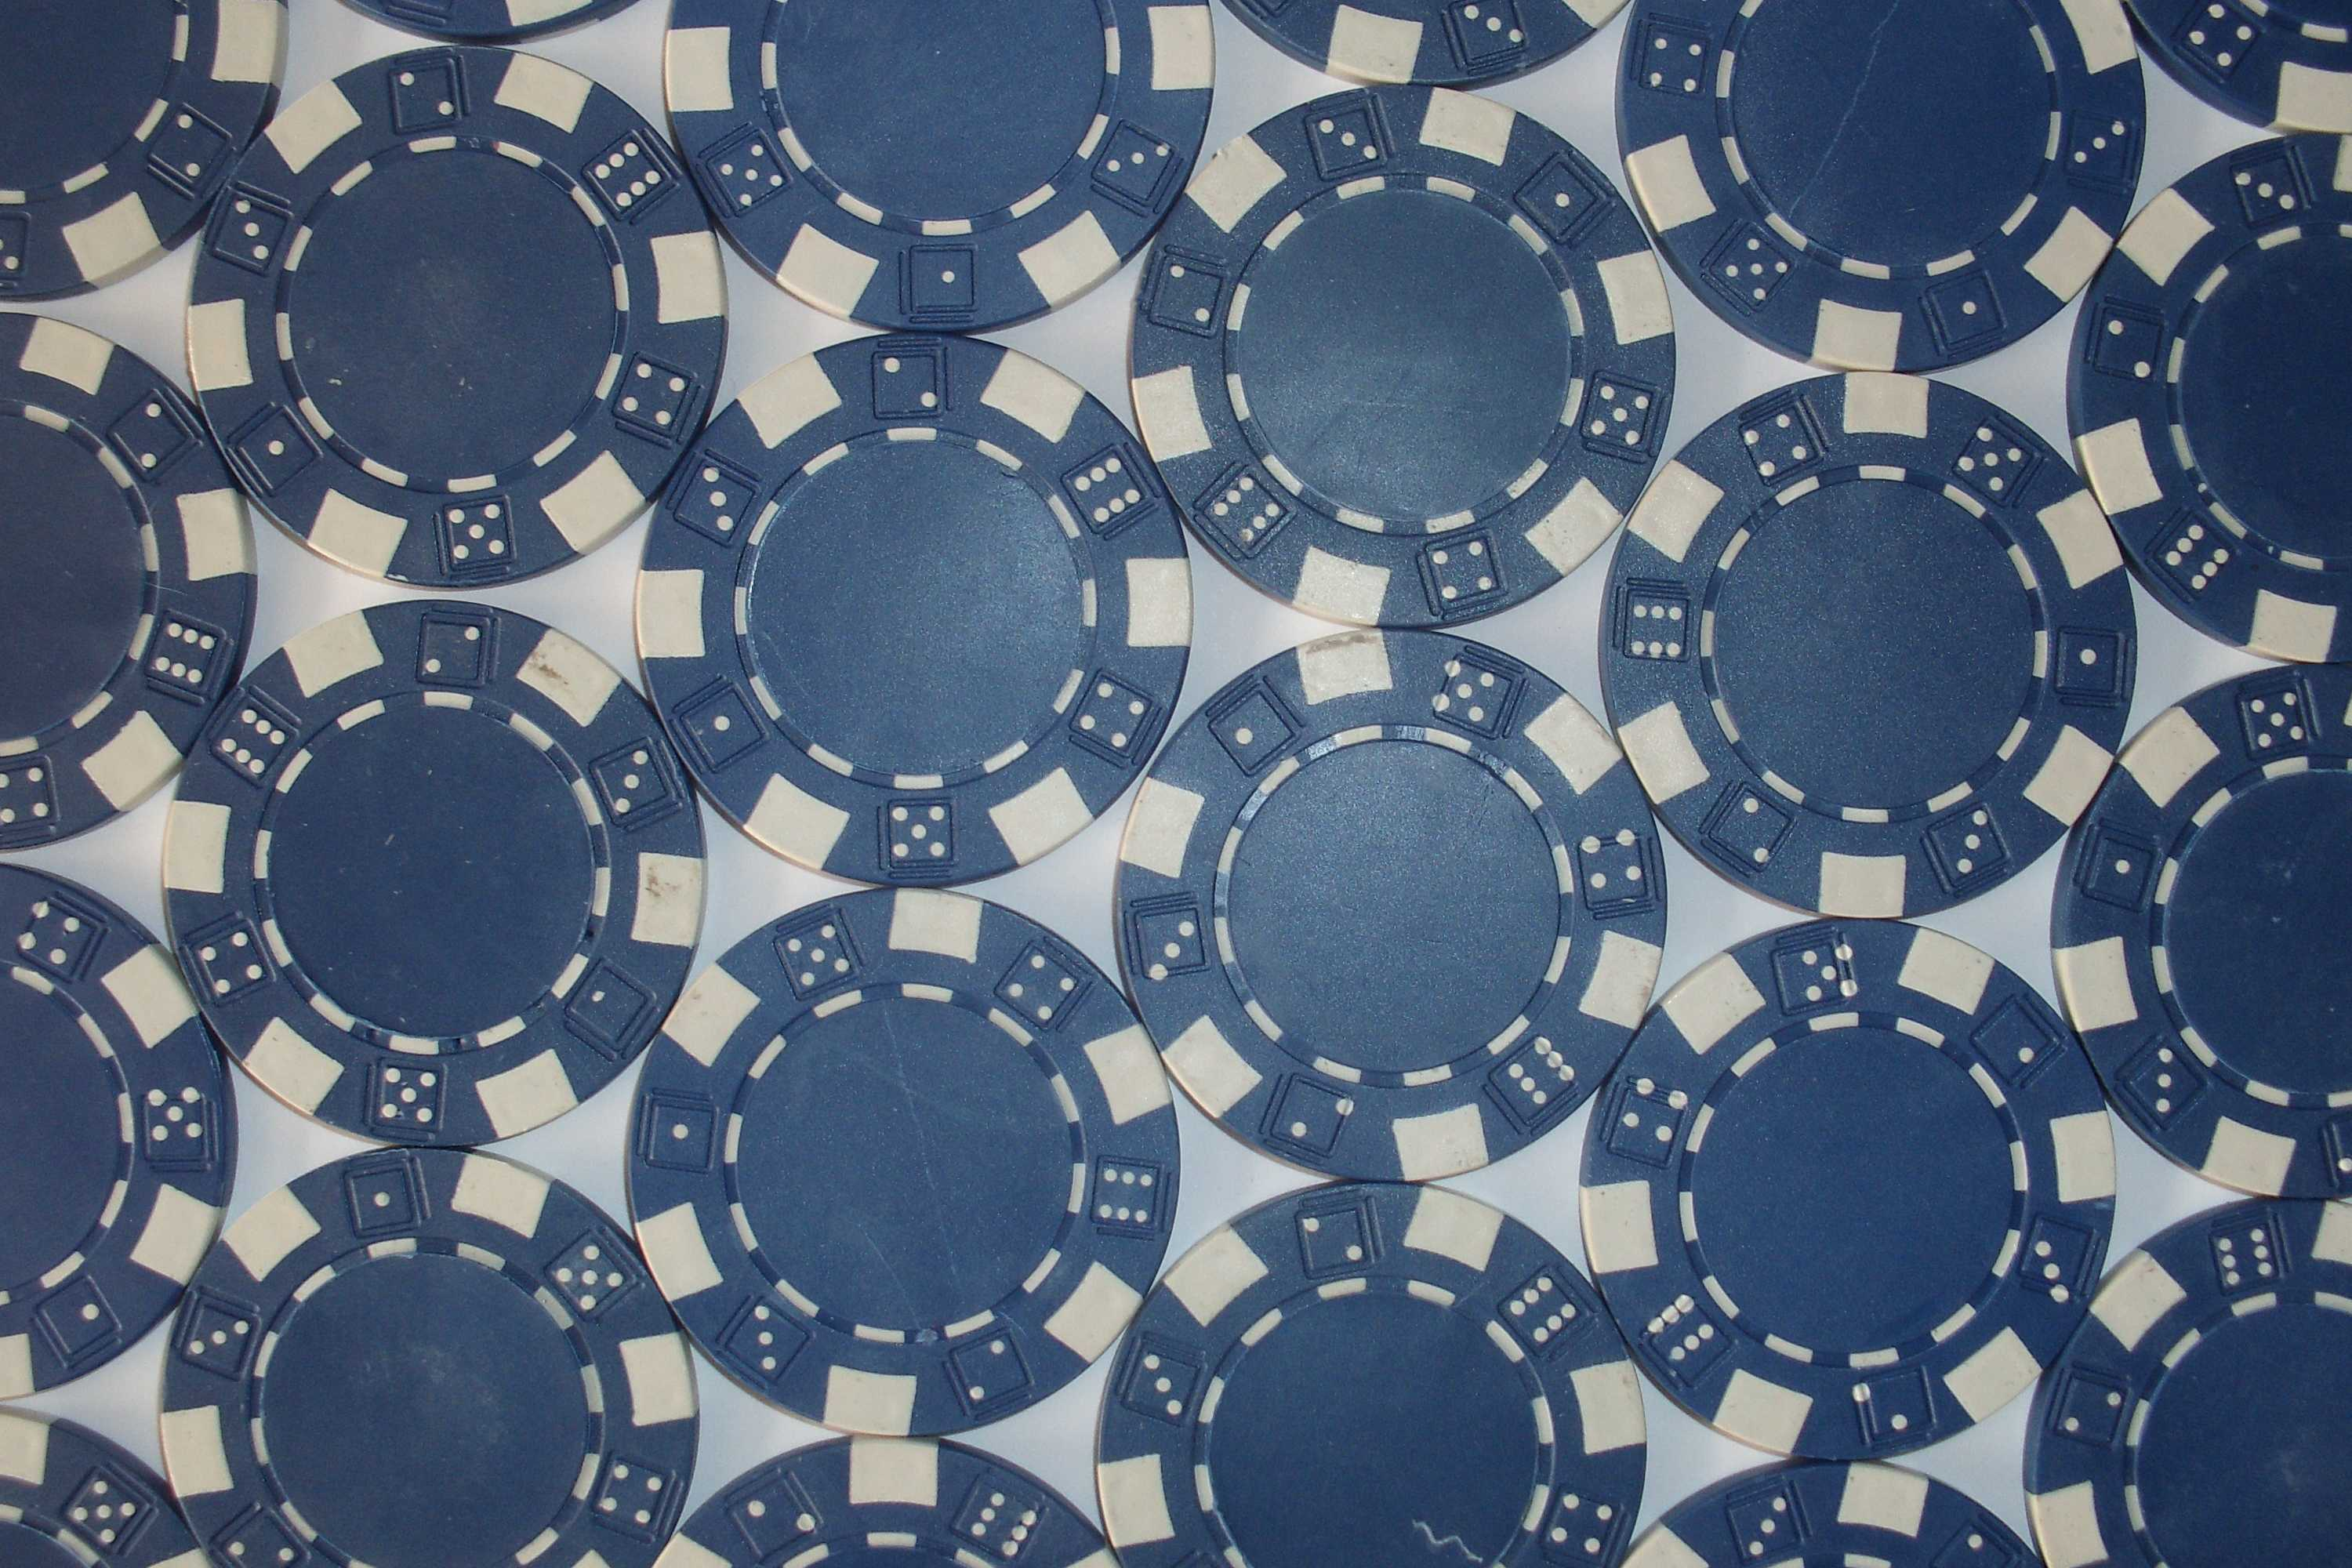
\includegraphics[height=4cm]{jetons_hex}\label{jh}}
 % \caption{Vierkante en hexagonale rangschikking met pokerjetons en hun voronoicellen.}  
%\end{figure}
\begin{columns}
        \begin{column}{0.4\textwidth}
    \begin{block}{Opdracht}
Probeer cirkels (munten, flippo's, pokerjetons ...) eens zodanig op een tafel te leggen dat er zo weinig mogelijk ruimte tussen de cirkels overblijft.
\end{block}
\end{column}
\begin{column}{0.4\textwidth}
      \only<2>{\begin{figure}[h]
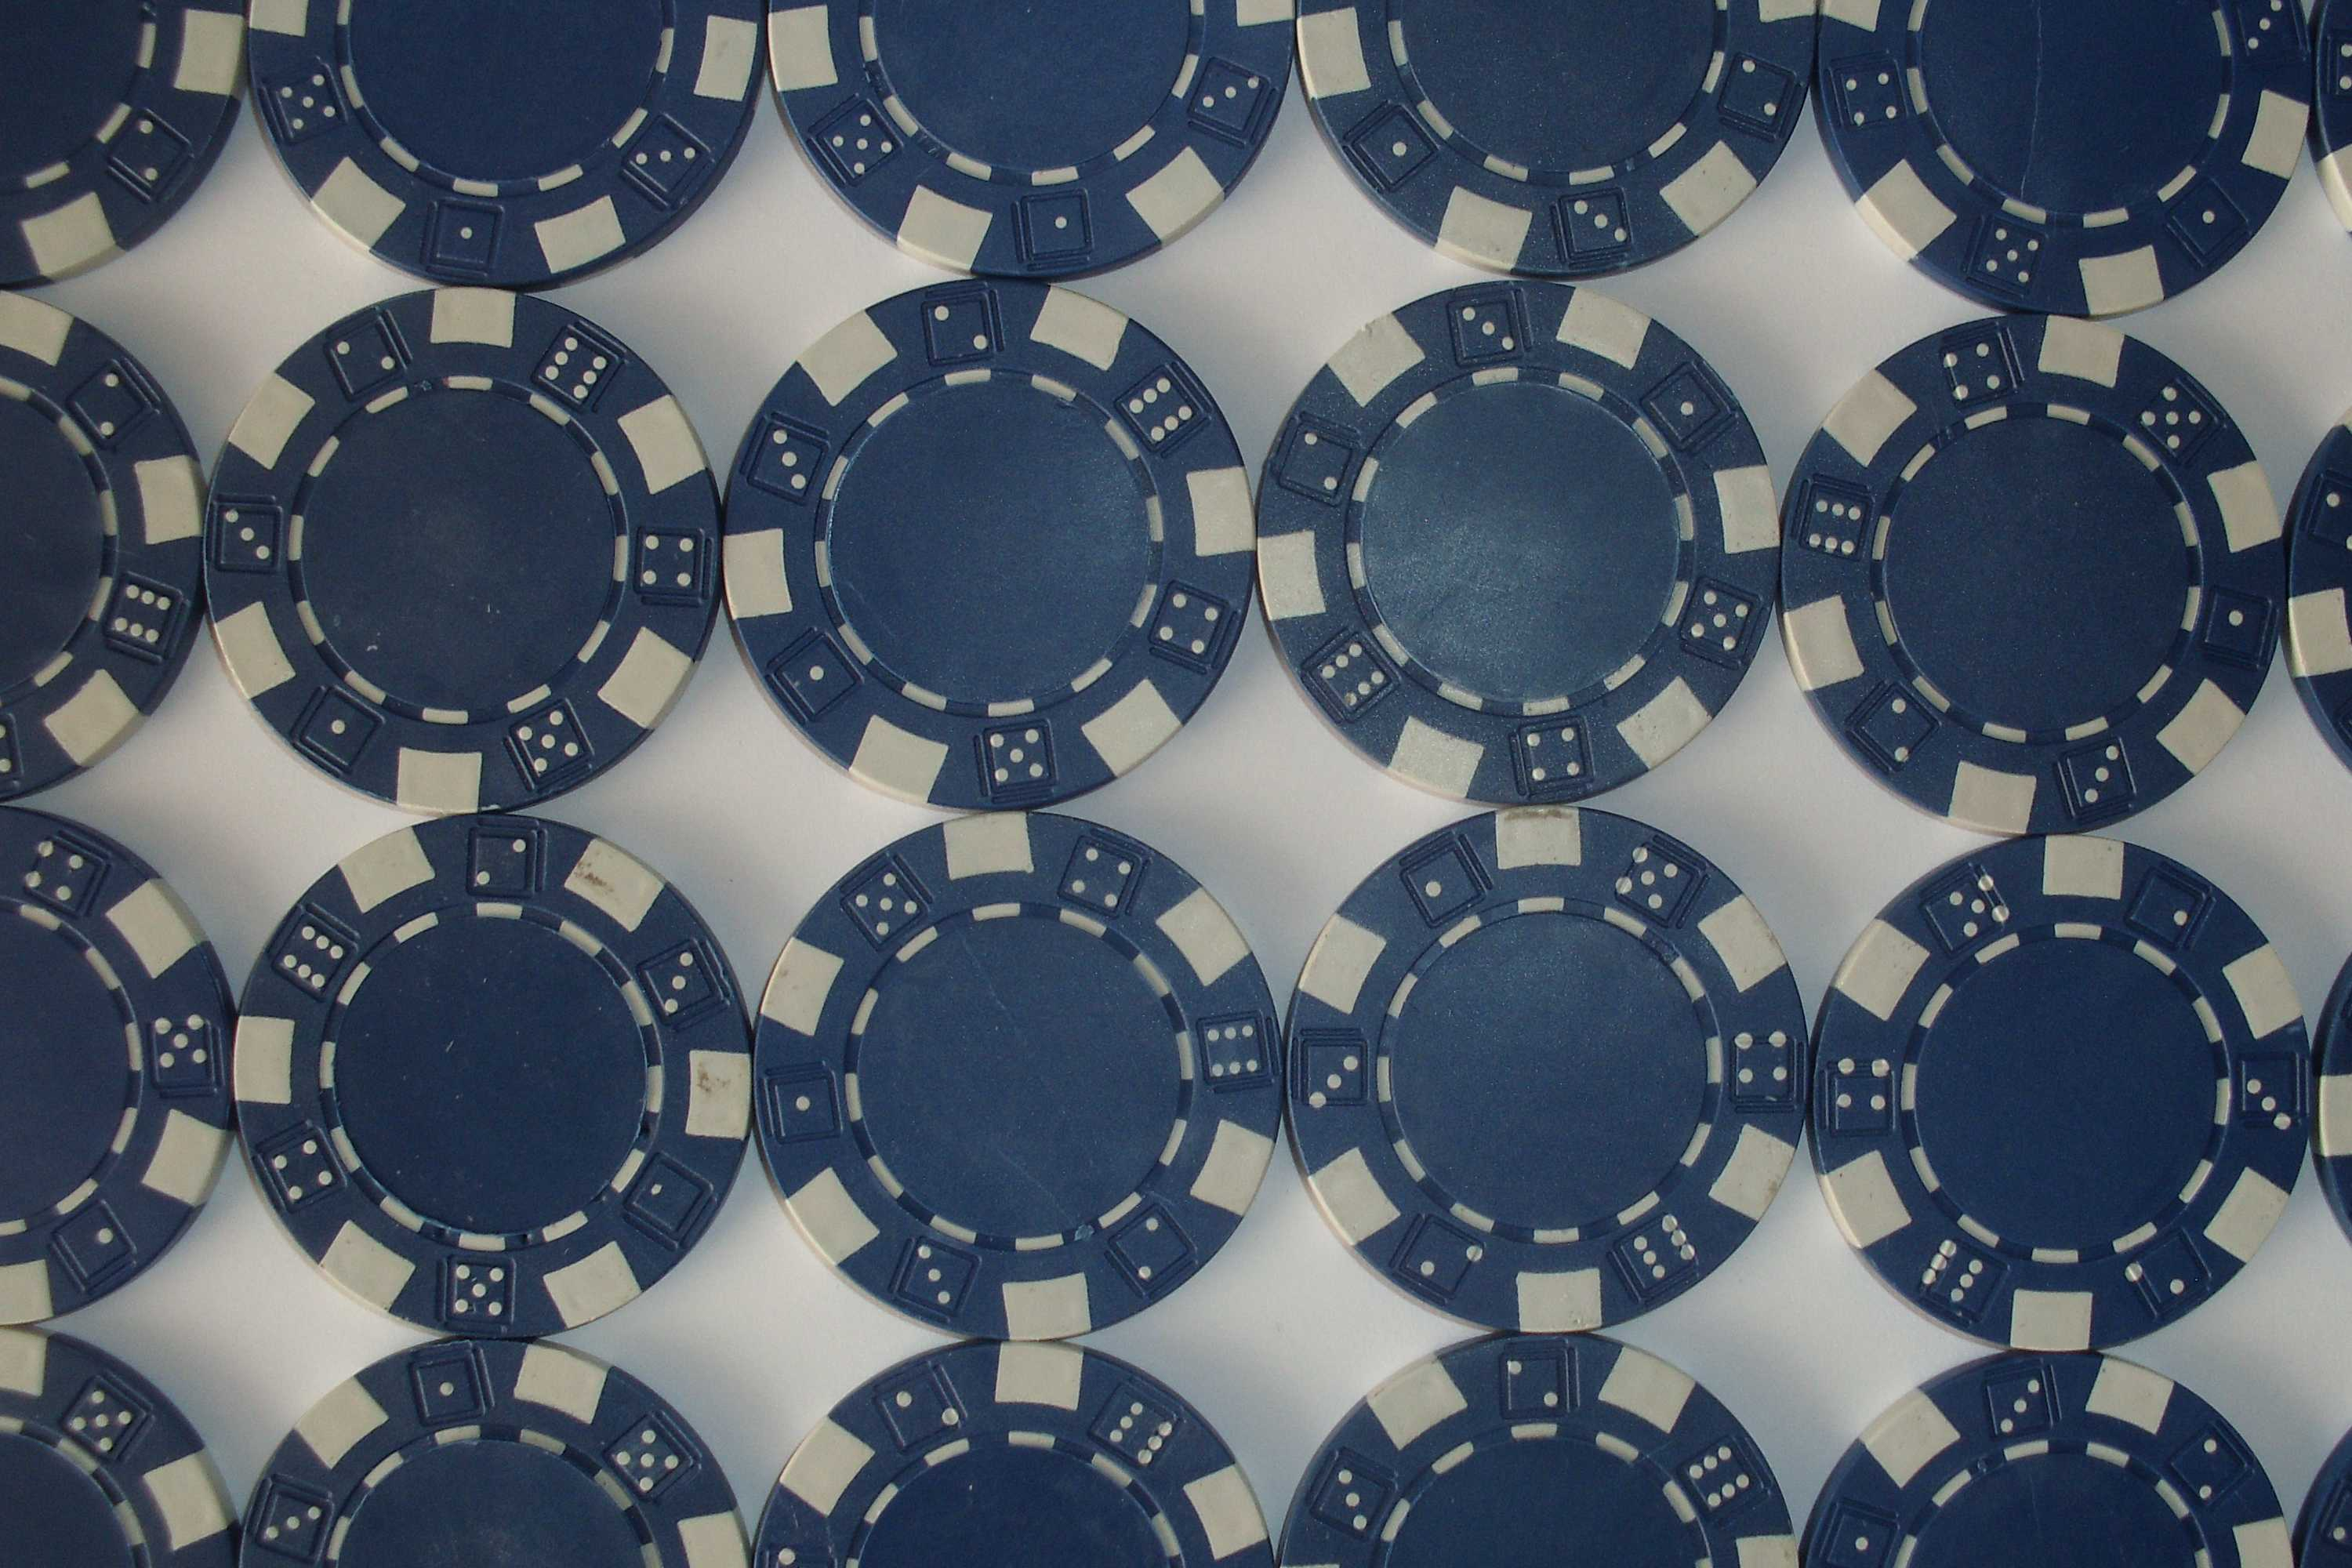
\includegraphics[width=\columnwidth]{jetons_sqr}
\end{figure}}
      \only<3>{\begin{figure}[h]
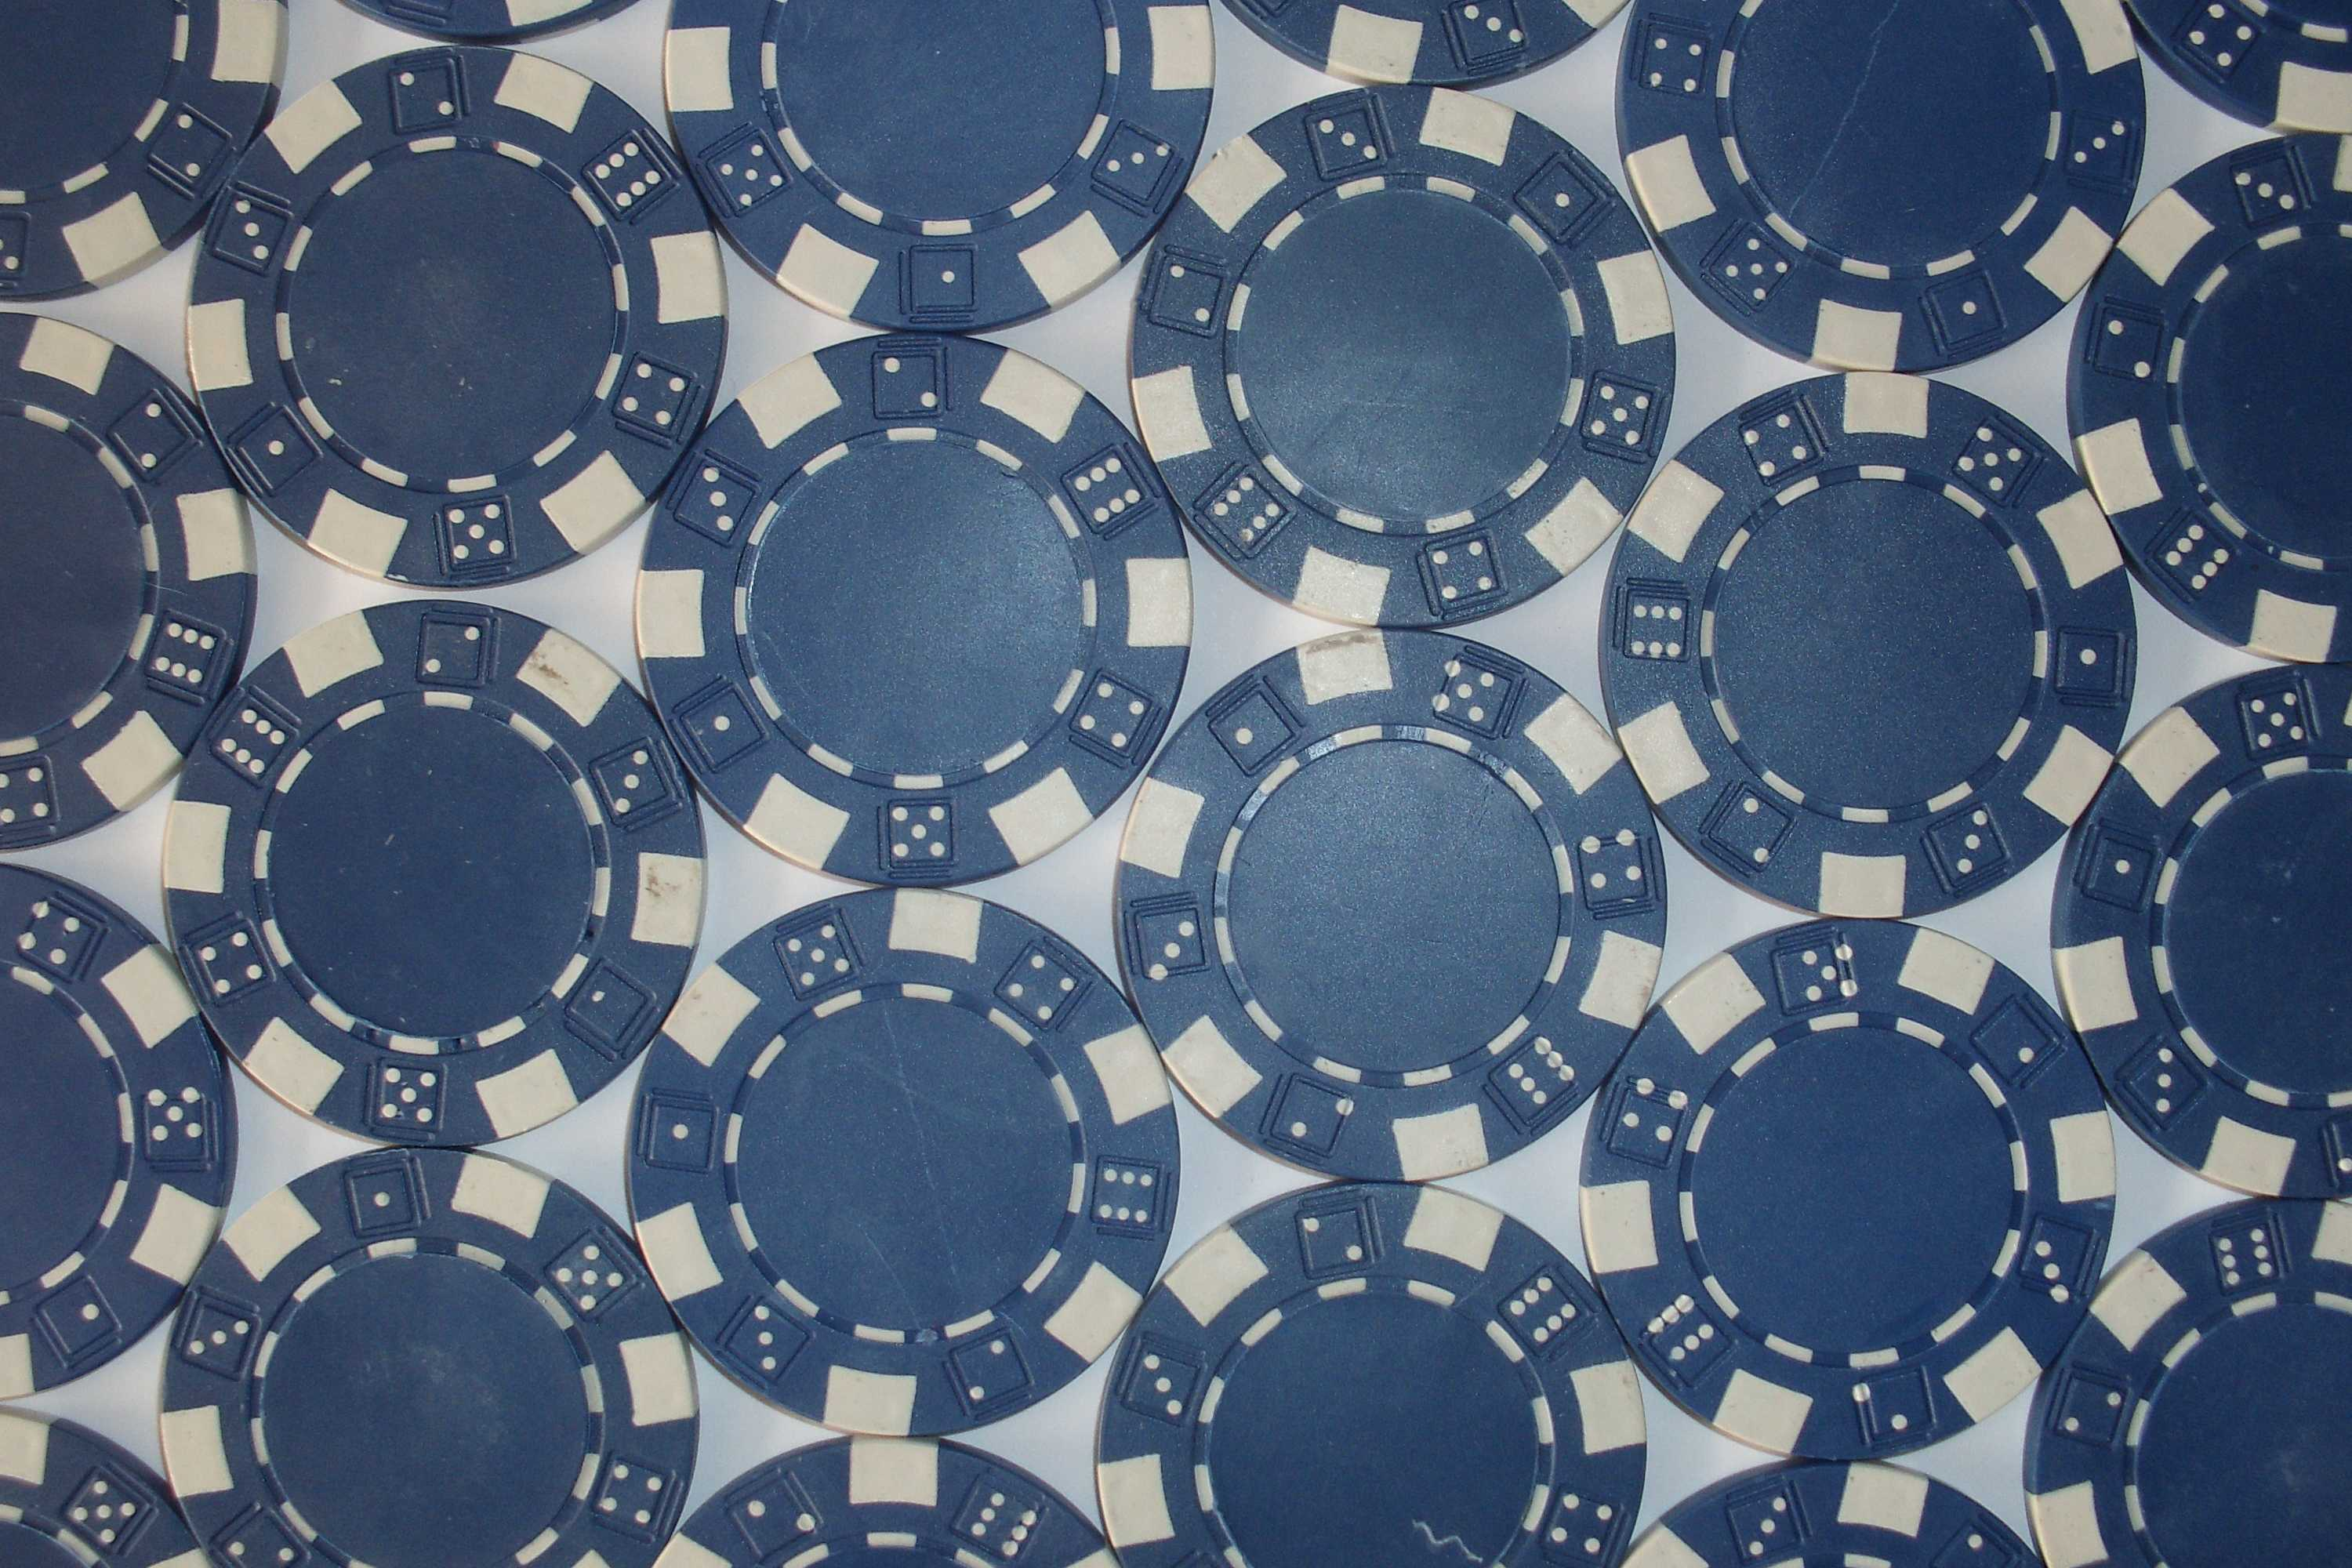
\includegraphics[width=\columnwidth]{jetons_hex}
\end{figure}}
    \end{column}
  \end{columns}  

\end{frame}

\begin{frame}
\begin{block}{Voronoicel}
De {\bf Voronoicel} van een cirkel is de verzameling van alle punten die dichter bij het middelpunt van deze cirkel liggen dan bij het middelpunt van elke andere cirkel in de schikking.
\end{block}


\begin{block}{Vraag}
Hoe ziet de Voronoicel eruit bij een vierkante rangschikking? Hoe ziet de Voronoicel eruit bij de hexagonale rangschikking?
\end{block}
\end{frame}


\begin{frame}
\begin{block}{Voronoicel}
De {\bf Voronoicel} van een cirkel is de verzameling van alle punten die dichter bij het middelpunt van deze cirkel liggen dan bij het middelpunt van elke andere cirkel in de schikking.
\end{block}


\begin{block}{Vraag}
\begin{columns}

        \begin{column}{0.4\textwidth}
Hoe ziet de Voronoicel eruit bij een vierkante rangschikking? Hoe ziet de Voronoicel eruit bij de hexagonale rangschikking?\end{column}
\begin{column}{0.4\textwidth}
     
      \only<1>{\begin{figure}[h]
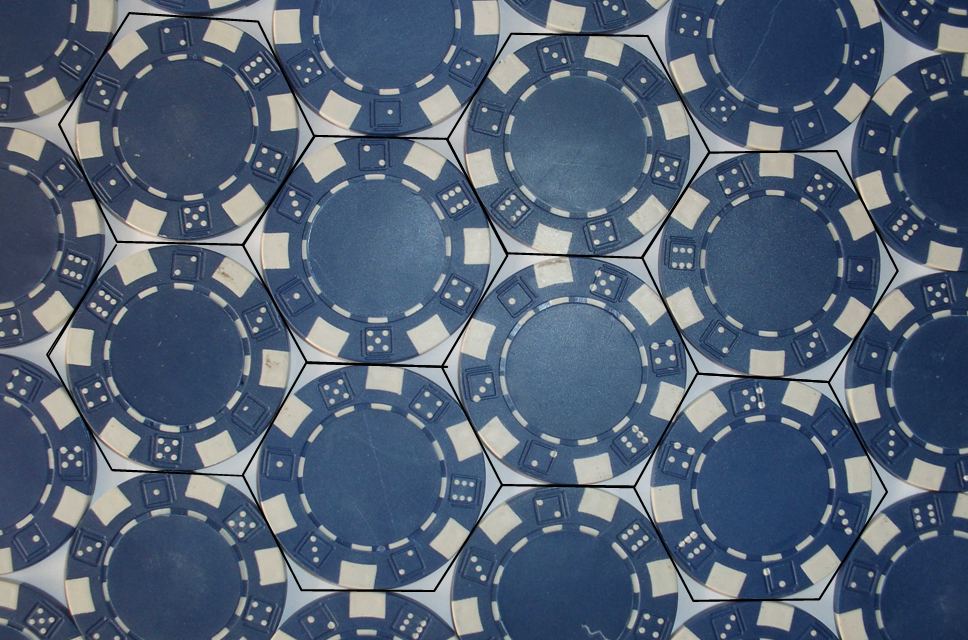
\includegraphics[width=\columnwidth]{voronoi_hex}
\end{figure}}
      \only<2>{\begin{figure}[h]
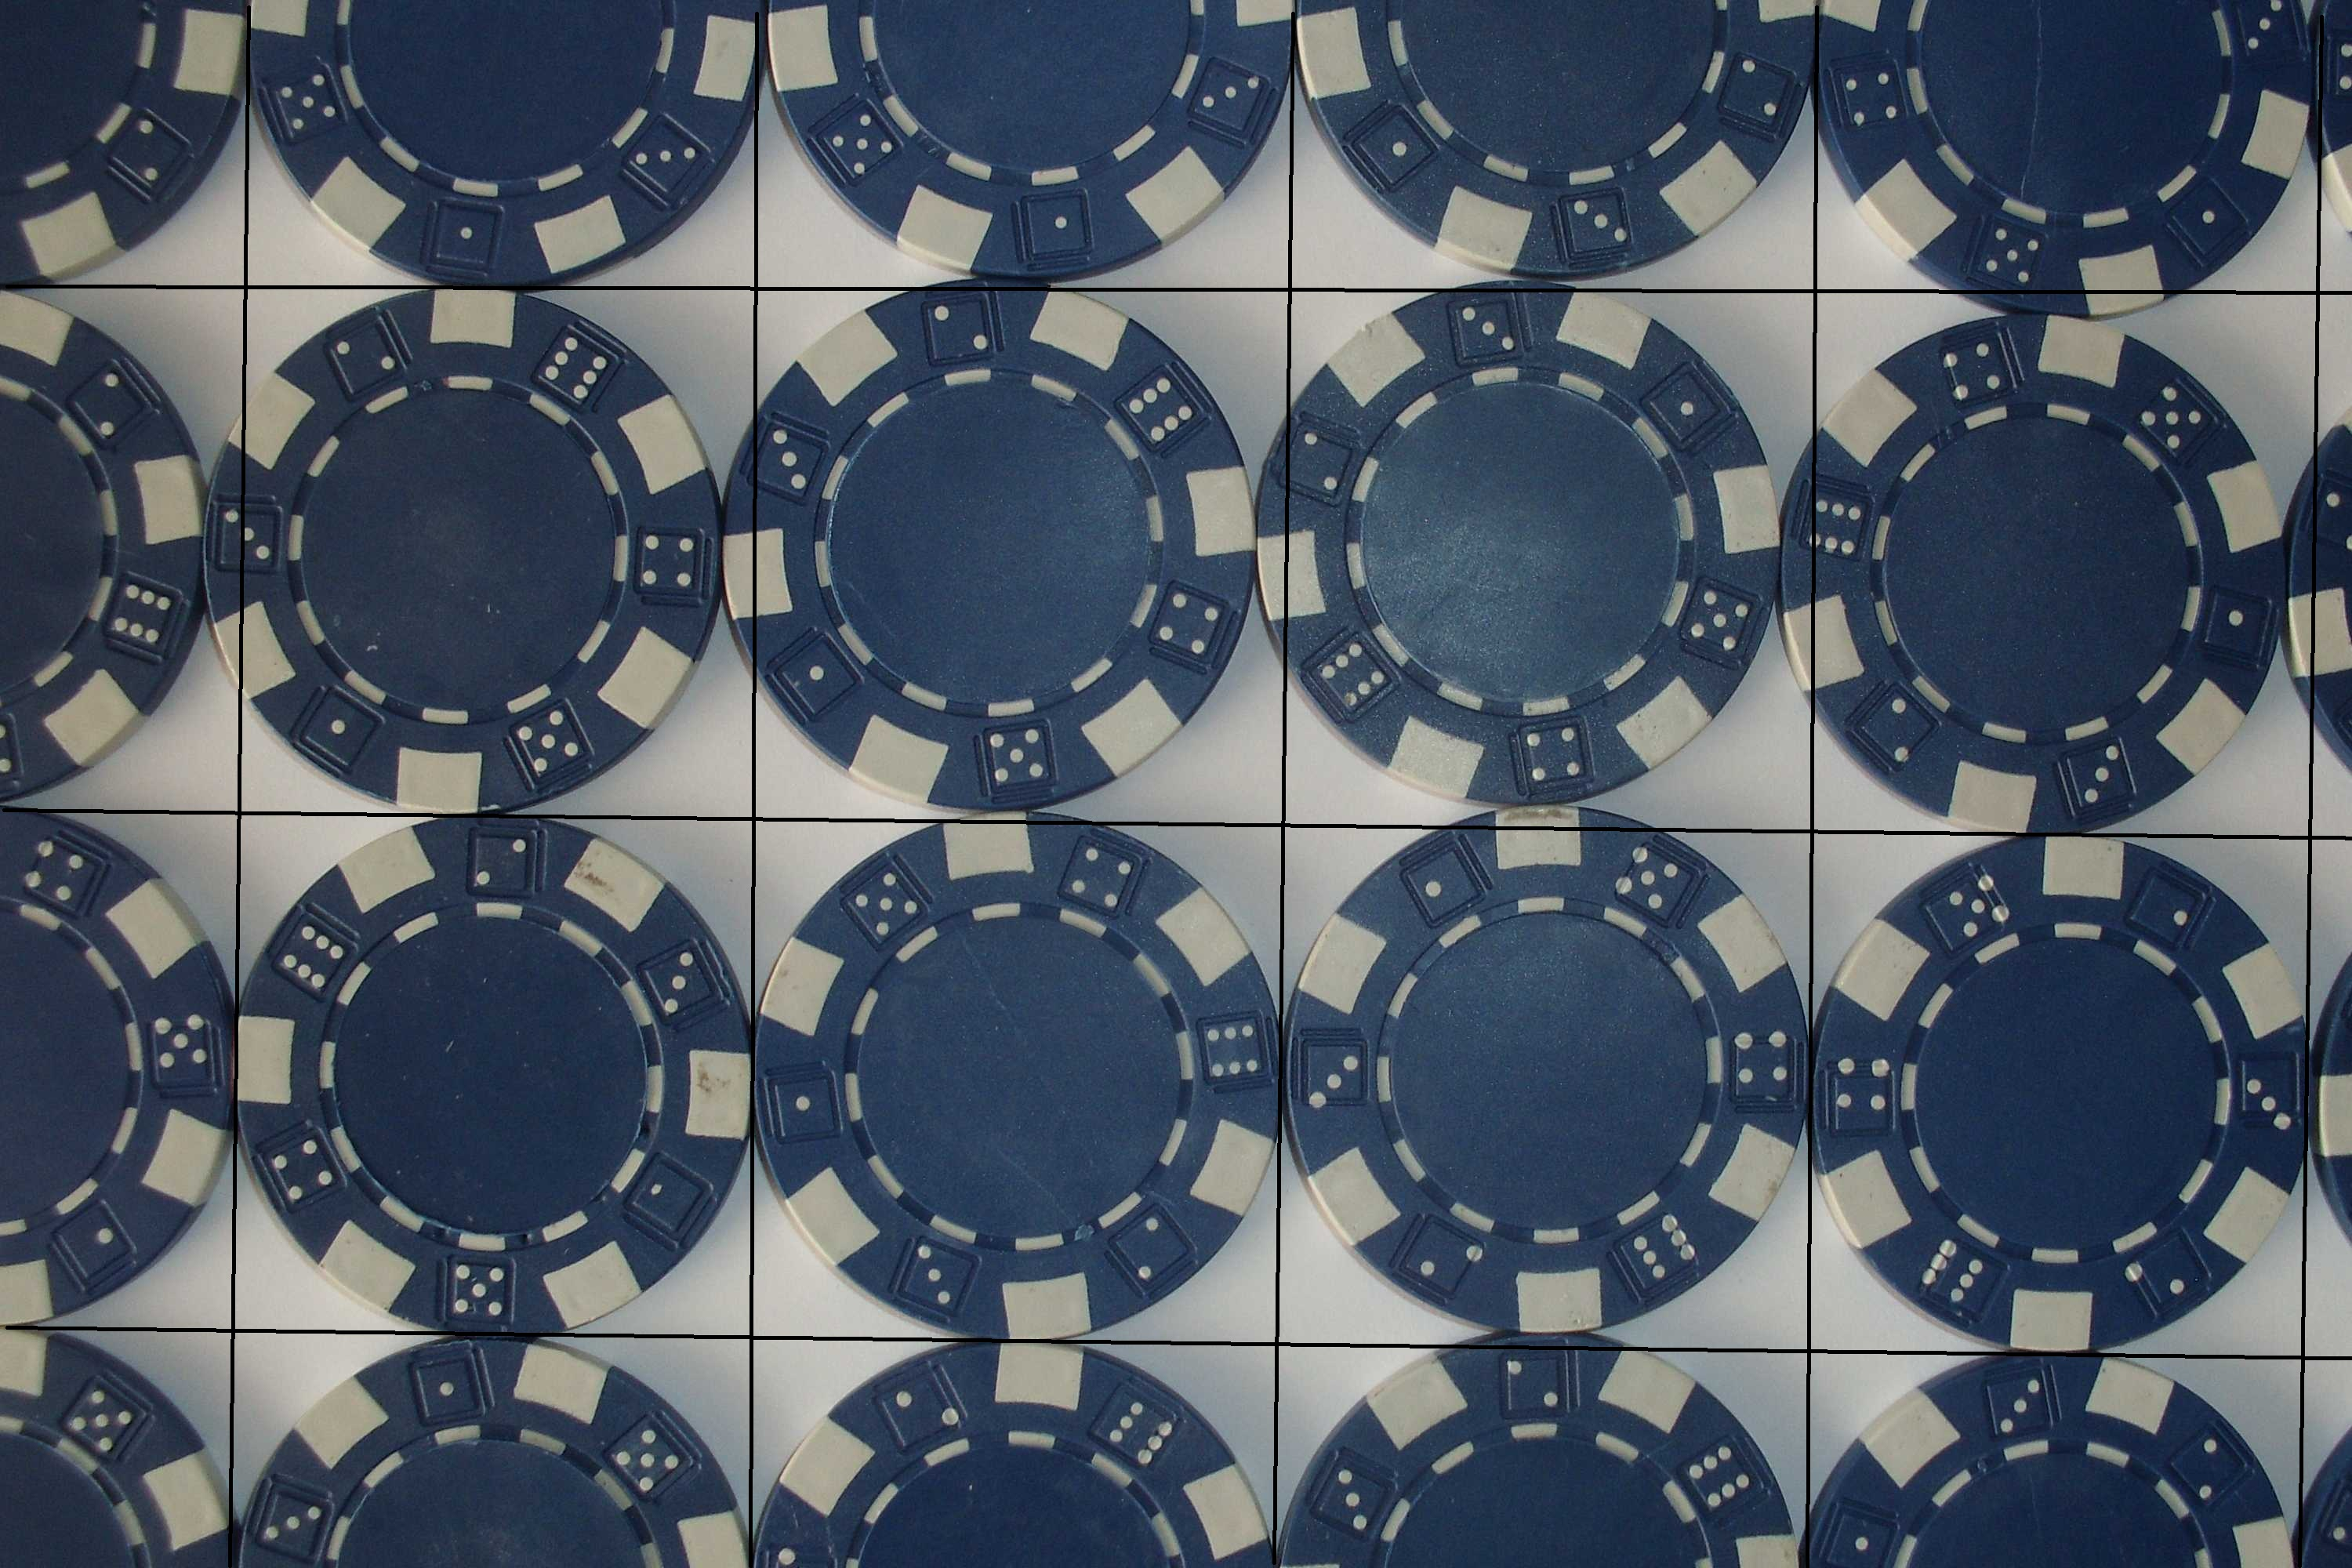
\includegraphics[width=\columnwidth]{voronoi_sqr}
\end{figure}}

    \end{column}
  \end{columns}  
\end{block}%Omdat in het tweede deel van de les en ook de volgende les de leerlingen zelf de effici�ntie zullen moeten berekenen is het goed om dit al eens klassikaal te doen.
%\begin{block}{Vraag}
%Hoe kan je de effici�ntie berekenen aan de hand van zo'n Voronoicel?
%\end{block}
\end{frame}

\begin{frame}
\begin{block}{Opdracht}
Bereken voor de vierkante en de hexagonale rangschikking de effici�ntie.
\end{block}
\begin{columns}
\begin{column}{0.6\textwidth}     
\begin{enumerate}
	\item Vierkante rangschikking: \\
 Effici�ntie = $\frac{\pi}{4}=0,78538...$
 \pause
	\item Hexagonale rangschikking:\\
	Effici�ntie = $\frac{\pi}{\sqrt{12}}=0.90689$
	%Dit is ook de meest effici�nte!!! -> Axel Thue heeft dit aangetoond en we geven in de cursus ook een kleine schets van het bewijs.
\end{enumerate}
\end{column}
\begin{column}{0.4\textwidth}     
     \only<2>{\begin{figure}[h]
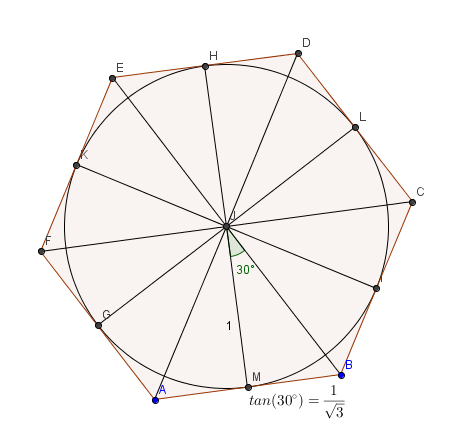
\includegraphics[width=\columnwidth]{hexagon}
\end{figure}}
   \end{column}
\end{columns}  
\end{frame}



